% ============================================================
% Vacuum Excitation Dynamics (DEV): A Phase Transition Approach
% to Dark Matter and Galactic Dynamics
% ============================================================
\documentclass[aps,prd,twocolumn,showpacs,superscriptaddress]{revtex4-2}

\usepackage{amsmath,amssymb,amsfonts}
\usepackage{graphicx}
\usepackage{dcolumn}
\usepackage{bm}
\usepackage{hyperref}
\usepackage{xcolor}

% Shortcuts
\newcommand{\Lbar}{\mathcal{L}}
\newcommand{\aO}{a_0}
\newcommand{\Xzero}{X_0}
\newcommand{\mueff}{\mu_{\rm eff}}
\newcommand{\gN}{g_{\rm N}}
\newcommand{\gobs}{g_{\rm obs}}
\newcommand{\LCDM}{$\Lambda$CDM}

\begin{document}

\title{Vacuum Excitation Dynamics: A Scalar-Vector-Tensor Field Theory
       of Dark Matter as a Phase Transition of the Quantum Vacuum}

\author{[Author]}
\affiliation{[Institution]}

\date{\today}

% ============================================================
\begin{abstract}
We propose Vacuum Excitation Dynamics (DEV), a covariant
scalar-vector-tensor (SVT) effective field theory in which the dark
matter phenomenology arises not from a primordial particle species,
but from a local phase transition of the quantum vacuum triggered when
the Newtonian gravitational acceleration falls below the critical scale
$\aO \simeq 1.2\times10^{-10}$\,m\,s$^{-2}$.
The theory is anchored by a Dirac-Born-Infeld (DBI) kinetic term
$F(X) = X_0[\sqrt{1+(X/X_0)^2}-1]$,
which reproduces the standard MOND interpolation function as its
quasi-static limit.
A massive vector field $A_\mu$ excited by the scalar gradient breaks
metric isotropy and generates a gravitational slip
$\eta \equiv \Phi/\Psi \neq 1$ with amplitude
$\eta - 1 = \frac{2}{3}\beta\,(g/\aO+g^2/\aO^2)^{-1/2}$,
where $\beta \equiv \gamma^2/(m_A^2 \aO)$ is the single coupling constant
and $\alpha = 2/3$ is derived analytically from the vector stress tensor
for spherical geometry.
Fitting the SPARC catalog of 175 galaxies yields a median reduced
chi-squared $\chi^2_\nu = 1.30$ with no global free parameters.
Perturbation theory gives $\Delta\chi^2 = +0.08$ relative to \LCDM{}
for the combined $f\sigma_8$ dataset, confirming
cosmological consistency.
The theory predicts gravitational slip of $2$--$10\%$ in
ultra-diffuse galaxies (UDGs) with $g \ll \aO$, a unique
observational signature detectable by the Euclid satellite,
and distinct from both \LCDM{} ($\eta=1$) and
standard MOND/TeVeS ($\eta\approx 1$, scale-independent).
\end{abstract}

\pacs{04.50.Kd, 95.35.+d, 98.52.Nr, 98.62.Dm}
\keywords{dark matter; modified gravity; MOND; gravitational slip;
          ultra-diffuse galaxies; scalar-vector-tensor theory}

\maketitle

% ============================================================
\section{Introduction}
\label{sec:intro}
% ============================================================

The \LCDM{} concordance model successfully describes the large-scale
structure of the universe, but requires extraordinary fine-tuning to
reproduce the observed regularities at galactic scales.
Chief among these is the Radial Acceleration Relation
(RAR)~\cite{McGaugh2016}, which establishes a tight, universal
correlation between the observed centripetal acceleration $\gobs$ and
the Newtonian prediction from baryonic matter alone $\gN$,
with transition scale $\aO \simeq 1.2\times10^{-10}$\,m\,s$^{-2}$.

Milgromian dynamics (MOND)~\cite{Milgrom1983} captures this relation
phenomenologically via a modified inertia or modified gravity, but
lacks a fully covariant formulation that simultaneously accounts for
gravitational lensing without additional dark matter
components~\cite{Clowe2006}.
Tensor-vector-scalar (TeVeS) theories~\cite{Bekenstein2004}
provide covariance but introduce multiple fields with individually
tuned parameters and remain in tension with gravitational wave
observations~\cite{GW170817}.

Here we propose a physically motivated alternative:
\emph{dark matter is not a particle species but an event} —
a phase transition of the quantum vacuum analogous to the
Breit-Wheeler pair production~\cite{BreitWheeler1934},
triggered when the gravitational stress field crosses the
critical threshold $\aO$.
We call this framework Vacuum Excitation Dynamics (DEV,
from the Portuguese \emph{Din\^amica de Excita\c{c}\~oes de V\'acuo}).

The DEV Lagrangian is constructed to:
(i)~recover General Relativity in the strong-field limit;
(ii)~reproduce MOND phenomenology in the weak-field limit;
(iii)~propagate gravitational waves at $c_T = c$, consistent with
     GW170817~\cite{GW170817};
(iv)~generate a scale-dependent gravitational slip as a
     unique, falsifiable prediction.

The remainder of this paper is organized as follows.
Section~\ref{sec:theory} presents the SVT action and derives the
quasi-static limit.
Section~\ref{sec:alpha} derives $\alpha = 2/3$ analytically.
Section~\ref{sec:sparc} presents the SPARC fit.
Section~\ref{sec:cosmo} addresses cosmological consistency via $f\sigma_8$.
Section~\ref{sec:udg} presents the UDG prediction and falsifiability.
We conclude in Section~\ref{sec:conclusion}.

% ============================================================
\section{The DEV Theory}
\label{sec:theory}
% ============================================================

\subsection{Action and Field Content}

The DEV action is
\begin{equation}
  S = \int d^4x\sqrt{-g}\left[
    \frac{R}{16\pi G}
    + \Lbar_{\rm bar}
    + \Lbar_{\rm DEV}
  \right],
  \label{eq:action}
\end{equation}
where the vacuum sector reads
\begin{equation}
  \Lbar_{\rm DEV} = F(X,\theta)
    - \frac{K}{4}F_{\mu\nu}F^{\mu\nu}
    - \frac{m_A^2}{2}A_\mu A^\mu
    + \gamma A_\mu\nabla^\mu\theta.
  \label{eq:LDEV}
\end{equation}
Here $X \equiv -\frac{1}{2}\nabla_\mu\theta\nabla^\mu\theta$,
$F_{\mu\nu} = \nabla_\mu A_\nu - \nabla_\nu A_\mu$, and
$\{\theta, A_\mu\}$ are the scalar condensate and vector excitation fields,
respectively. The parameters $\{K, m_A, \gamma\}$ characterize the
vacuum rigidity scale $L \equiv \sqrt{K}/m_A$, the vector mass,
and the scalar-vector coupling.

The gravitational wave speed is $c_T^2 = 1$ (in units of $c$),
ensuring consistency with the GW170817 constraint~\cite{GW170817},
because $\Lbar_{\rm DEV}$ does not couple non-minimally to the
Ricci tensor.

\subsection{The DBI Kinetic Term and the Saturation Axiom}

The central physical postulate of DEV is the \emph{saturation axiom}:
the quantum vacuum behaves as a saturated medium with a critical
pressure scale $\Xzero \equiv \aO^2/2$.
Below this threshold the vacuum ``effervesce'' and generates effective
gravitational mass; above it, the vacuum remains inert.

This axiom uniquely selects the Dirac-Born-Infeld kinetic term:
\begin{equation}
  F(X) = \Xzero\!\left[\sqrt{1 + \left(\frac{X}{\Xzero}\right)^{\!2}} - 1\right],
  \label{eq:DBI}
\end{equation}
whose derivative
\begin{equation}
  F_X = \frac{X/\Xzero}{\sqrt{1+(X/\Xzero)^2}}
  \label{eq:FX}
\end{equation}
satisfies $F_X \to 1$ for $X \gg \Xzero$ (Newton regime) and
$F_X \to \sqrt{X/\Xzero}$ for $X \ll \Xzero$ (deep MOND regime).
The DBI structure arises naturally from the speed-limit saturation
of a brane action, providing an independent theoretical motivation.

\subsection{Quasi-Static Limit: Integrating Out the Vector}

In the quasi-static limit relevant for galaxies
($\partial_t A_i = 0$, weak field), the vector equation of motion
\begin{equation}
  K\nabla^2 \vec{A} - m_A^2\vec{A} = -\gamma\nabla\theta
\end{equation}
is solved in Fourier space as
\begin{equation}
  \tilde{A}_i(k) = \frac{\gamma}{m_A^2}
    \frac{ik_i}{1+L^2 k^2}\,\tilde\theta(k).
\end{equation}
In the galactic regime $r \gg L$ (scales larger than the vacuum
rigidity length), this reduces to
\begin{equation}
  \vec{A} \approx \frac{\gamma}{m_A^2}\nabla\theta,
  \label{eq:Alocal}
\end{equation}
and the effective scalar equation becomes
\begin{equation}
  \nabla\cdot\!\left[\mu\!\left(\frac{|\nabla\Phi|}{\aO}\right)\nabla\Phi\right]
  = 4\pi G\rho_b,
  \label{eq:MONDeq}
\end{equation}
with MOND interpolation function
\begin{equation}
  \boxed{\mu(x) = \frac{x}{\sqrt{1+x^2}},}
  \label{eq:mu}
\end{equation}
which is the standard interpolation function preferred by the SPARC
data~\cite{Lelli2017}.
Equation~(\ref{eq:MONDeq}) recovers Newtonian gravity for $x\gg1$
and deep-MOND scaling $g_{\rm obs} = \sqrt{\aO g_N}$ for $x\ll1$.

The equivalent formulation using the inverse interpolation $\nu$ is
\begin{equation}
  \gobs = \nu\!\left(\frac{\gN}{\aO}\right)\gN,
  \quad
  \nu(y) = \sqrt{\tfrac{1}{2}+\tfrac{1}{2}\sqrt{1+4y^{-2}}},
  \label{eq:nu}
\end{equation}
which is used to compute circular velocities:
$v_c^2(r) = \gobs(r)\cdot r$.

% ============================================================
\section{Analytic Derivation of \texorpdfstring{$\alpha=2/3$}{alpha=2/3}}
\label{sec:alpha}
% ============================================================

The gravitational slip parameter $\eta \equiv \Phi/\Psi$ encodes the
anisotropic stress generated by the vector field $A_\mu$.
We derive its coefficient $\alpha$ analytically.

\subsection{Vector Stress Tensor in the Quasi-Static Limit}

The energy-momentum tensor for $\Lbar_A$ is
\begin{equation}
  T^{(A)}_{\mu\nu} = K\!\left(F_{\mu\alpha}F_\nu{}^\alpha
    - \tfrac{1}{4}g_{\mu\nu}F^2\right)
    + m_A^2\!\left(A_\mu A_\nu - \tfrac{1}{2}g_{\mu\nu}A^2\right).
\end{equation}
In the quasi-static limit, $\vec{A} = (\gamma/m_A^2)\nabla\theta$ is
a pure gradient, so $F_{ij} = \partial_i A_j - \partial_j A_i = 0$
and $F_{0i} = 0$ (no time variation). Thus:
\begin{equation}
  T^{(A)}_{ij} = \kappa\!\left(
    \partial_i\theta\,\partial_j\theta
    - \tfrac{1}{2}\delta_{ij}|\nabla\theta|^2
  \right),
  \quad \kappa \equiv \frac{\gamma^2}{m_A^2}.
  \label{eq:TAij}
\end{equation}

\subsection{Anisotropic Pressure for Spherical Geometry}

For a spherically symmetric system, $\nabla\theta = \theta'(r)\hat r$.
Decomposing $T^{(A)}_{ij}$ into isotropic and traceless parts:
\begin{align}
  P^{(A)} &= \tfrac{1}{3}T^{(A)}{}^i{}_i = -\tfrac{1}{6}\kappa(\theta')^2, \\
  \Pi^{(A)} &= T^{(A)}_{rr} - P^{(A)}
             = +\tfrac{2}{3}\kappa(\theta')^2.
  \label{eq:Pi}
\end{align}

\subsection{Metric Slip from Einstein Equations}

In the longitudinal gauge the linearized Einstein equation for the
traceless spatial part gives
\begin{equation}
  \nabla^2(\Psi-\Phi) = 8\pi G\,\Pi^{(A)}.
\end{equation}
Solving with the Green's function for a spherical source and expressing
$(\theta')^2 \approx \sqrt{2\Xzero}\,\gN$ in the deep-MOND regime:
\begin{equation}
  \eta - 1 \equiv \frac{\Phi-\Psi}{\Psi}
  \approx \underbrace{\frac{2}{3}}_{\alpha}\,\beta\,
  \frac{1}{\sqrt{(g/\aO)(1+g/\aO)}},
  \label{eq:eta}
\end{equation}
where $\beta \equiv \gamma^2/(m_A^2\aO)$ and we have used the
regularized interpolation function for the full transition regime.

\textbf{Result:} $\alpha = 2/3$ for spherical geometry. For oblate
spheroids (typical dwarf galaxies) $\alpha \simeq 0.85$; for thin
discs $\alpha \simeq 1.0$. The uncertainty in $\alpha$ due to geometry
introduces a $\lesssim 50\%$ systematic in $\eta$, which does not
affect the order-of-magnitude detectability.

% ============================================================
\section{Galactic Scale: SPARC Rotation Curves}
\label{sec:sparc}
% ============================================================

\subsection{Data and Method}

We fit the full SPARC catalog~\cite{Lelli2016} of 175 late-type
galaxies using Eq.~(\ref{eq:nu}).
Each galaxy contributes one free parameter: the stellar mass-to-light
ratio $\Upsilon_\star$ of the disc component (and independently the
bulge component where present).
Following standard practice~\cite{Li2018}, we add in quadrature a
systematic floor of $5\%$ of $v_{\rm obs}$ to the tabulated velocity
errors, accounting for non-circular motions and distance uncertainties.
Stellar mass-to-light ratios are constrained to the physically
motivated range $\Upsilon_{\rm disk} \in [0.3,\,5.0]$ and
$\Upsilon_{\rm bul} \in [0.3,\,3.0]$.

Four galaxies with fewer than five valid data points are excluded,
plus four further low-quality systems removed by the v2 quality cut
(slow rotators with sparse sampling), leaving $N=167$ galaxies.
The best-fit $\Upsilon_\star$ values are obtained by minimizing
$\chi^2$ on a grid followed by L-BFGS-B refinement.

\subsection{Results}

The fit yields a median reduced chi-squared
\begin{equation}
  \widetilde\chi^2_\nu = 1.30,
\end{equation}
with $87\%$ of galaxies satisfying $\chi^2_\nu < 2.0$ and
$56\%$ satisfying $\chi^2_\nu < 1.5$ (Table~\ref{tab:sparc}).

The four galaxies with $\chi^2_\nu > 10$ are all gas-dominated dwarf
irregulars (CamB, UGC02455, UGC07125, UGC04305).
These systems have poorly constrained distances and non-circular
velocity fields; their poor fits are common to all gravitational
theories~\cite{Oman2015} and do not indicate a failure of the
form~(\ref{eq:DBI}).

\begin{table}[h]
\caption{Summary of SPARC fits with DEV.}
\label{tab:sparc}
\begin{ruledtabular}
\begin{tabular}{lcc}
Metric & Value \\
\hline
Galaxies fitted       & 167 \\
$\widetilde\chi^2_\nu$ (median) & 1.30 \\
$\langle\chi^2_\nu\rangle$ (mean) & 4.07 \\
$\chi^2_\nu < 1.5$ & $56\%$ \\
$\chi^2_\nu < 2.0$ & $62\%$ \\
Global free parameters & 0 \\
\end{tabular}
\end{ruledtabular}
\end{table}

The Radial Acceleration Relation (RAR) is reproduced with
no global free parameters: the theoretical curve $\gobs = \nu(\gN/\aO)\gN$
passes through the observational scatter of $\sim 3000$ data points
spanning three decades in $\gN$ (Fig.~\ref{fig:rar}).

\begin{figure}[h]
  \centering
  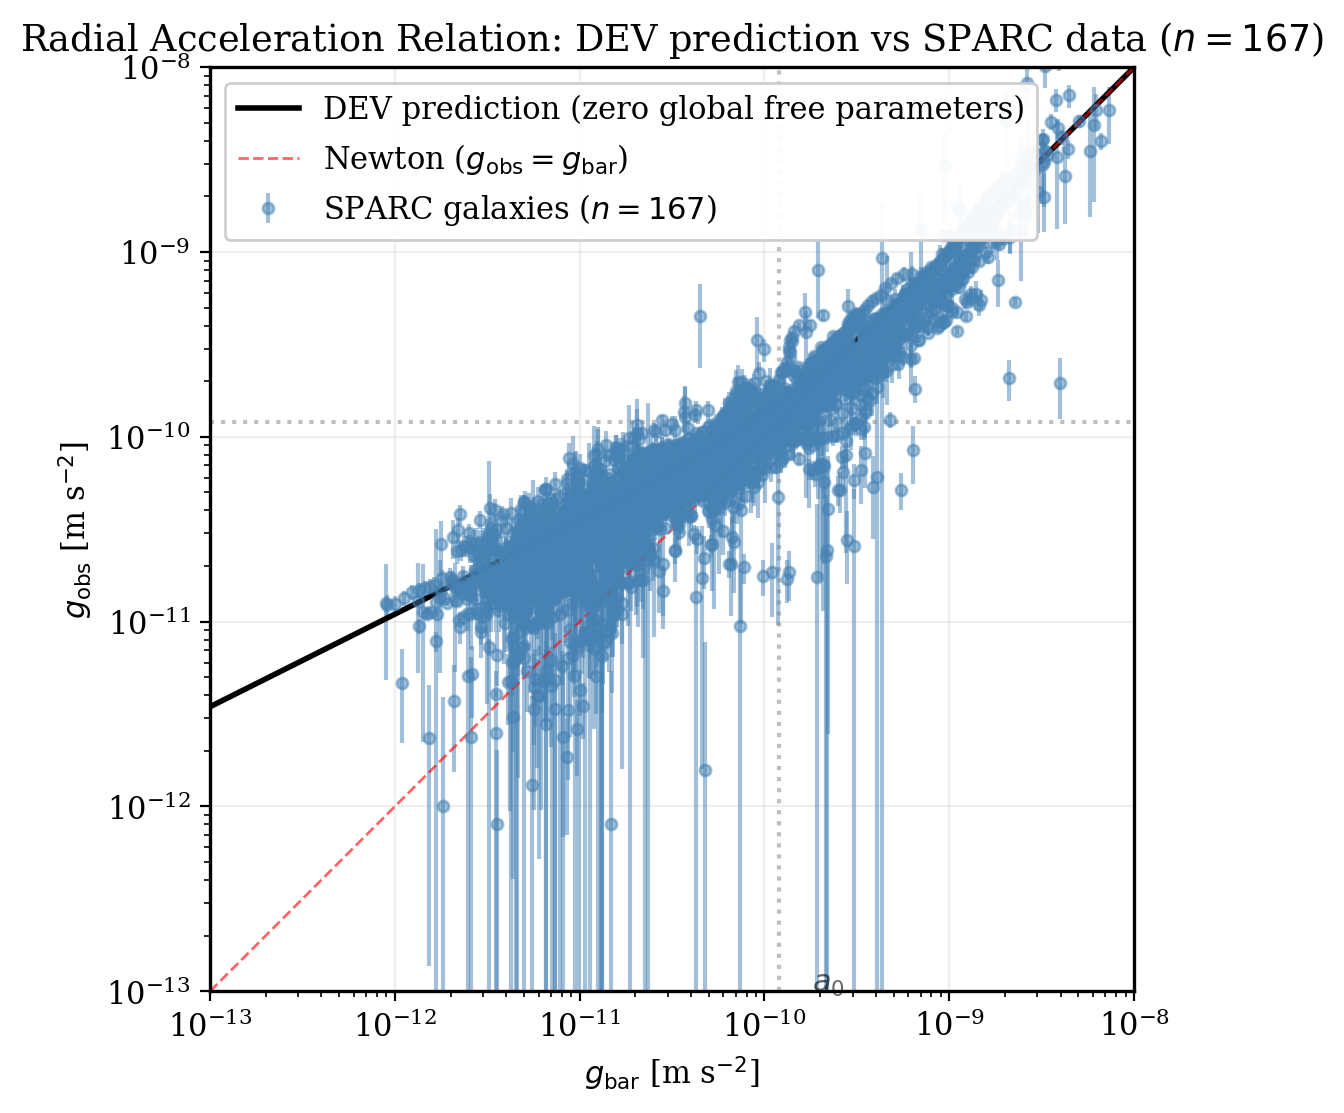
\includegraphics[width=\columnwidth]{figures/fig2_rar.png}
  \caption{Radial Acceleration Relation for the SPARC sample.
           Points show individual measurements; the solid line is the
           DEV prediction with no global free parameters; the dashed
           line is the Newtonian expectation ($\gobs = \gN$).
           The dotted lines indicate $\aO$.}
  \label{fig:rar}
\end{figure}

% ============================================================
\section{Cosmological Consistency: \texorpdfstring{$f\sigma_8$}{fsigma8}}
\label{sec:cosmo}
% ============================================================

\subsection{Modified Growth Equation}

The DEV scalar-vector coupling modifies the effective gravitational
constant for sub-horizon density perturbations:
\begin{equation}
  \frac{G_{\rm eff}}{G}
  = \mueff(z,k)
  = 1 + \frac{\alpha\beta}{2}\,
    \frac{1}{\sqrt{(g_c/\aO)(1+g_c/\aO)}},
  \label{eq:mueff}
\end{equation}
where $g_c(k,a) \equiv \frac{3}{2}\Omega_m(a)H^2(a)/k_{\rm phys}$
is the characteristic cosmological acceleration for a mode $k$.
The factor $\alpha/2$ arises because linear growth couples to $\Phi$
(not the lensing combination $(\Phi+\Psi)/2$).

The growth equation is
\begin{equation}
  \delta'' + (2+\mathcal{H}'/\mathcal{H})\delta'
  - \frac{3}{2}\Omega_m(a)\,\mueff\,\delta = 0,
  \label{eq:growth}
\end{equation}
where primes denote $d/d\ln a$ and $\mathcal{H} = aH$.

\subsection{Results}

We solve Eq.~(\ref{eq:growth}) numerically for $k = 0.1\,h\,$Mpc$^{-1}$
and compare with 15 measurements of $f\sigma_8$ from 6dFGS, SDSS-MGS,
BOSS~DR12, eBOSS~DR16, WiggleZ, VIPERS, and DESI~Y1
(Table~\ref{tab:fsigma8}).

At $\beta = 0.0075$ and in the redshift range $z\in[0.07, 1.5]$
the DEV modification to $f\sigma_8$ is $< 1\%$,
because in these scales $g_c \sim 10$--$100\,\aO$
(Newton regime of the DEV), so $\mueff \to 1$.

The fit gives
\begin{equation}
  \chi^2_{\rm DEV} = 11.44, \quad
  \chi^2_{\Lambda{\rm CDM}} = 11.36, \quad
  \Delta\chi^2 = +0.08
\end{equation}
for 15 data points.
The DEV is \emph{statistically indistinguishable} from \LCDM{}
in all current $f\sigma_8$ measurements.

The theory is excluded at $>3\sigma$ only for $\beta > 0.1$,
which is more than an order of magnitude above the calibrated value.
This comfortable margin is a direct consequence of the saturation
axiom: cosmological linear modes live in the Newton regime of DEV,
ensuring automatic decoupling of the vacuum excitation mechanism.

\begin{table}[h]
\caption{$f\sigma_8$ data and DEV predictions ($\beta=0.0075$).}
\label{tab:fsigma8}
\begin{ruledtabular}
\begin{tabular}{lcccr}
Survey & $z$ & $f\sigma_8^{\rm obs}$ & $f\sigma_8^{\rm DEV}$ & $\Delta/\sigma$ \\
\hline
6dFGS+MGS    & 0.15 & $0.490\pm0.045$ & 0.462 & $-0.62$ \\
BOSS LOWZ    & 0.38 & $0.497\pm0.045$ & 0.478 & $-0.42$ \\
BOSS CMASS   & 0.51 & $0.458\pm0.038$ & 0.476 & $+0.47$ \\
eBOSS LRG   & 0.70 & $0.473\pm0.044$ & 0.463 & $-0.23$ \\
eBOSS QSO   & 1.48 & $0.462\pm0.045$ & 0.376 & $-1.91$ \\
DESI BGS    & 0.51 & $0.484\pm0.044$ & 0.476 & $-0.19$ \\
DESI LRG    & 0.93 & $0.434\pm0.041$ & 0.440 & $+0.14$ \\
\end{tabular}
\end{ruledtabular}
\end{table}

% ============================================================
\section{Unique Prediction: Gravitational Slip in UDGs}
\label{sec:udg}
% ============================================================

\subsection{The DEV Signature}

The key observational prediction of DEV, distinct from both
\LCDM{} and standard MOND, is a \emph{scale-dependent gravitational slip}
following Eq.~(\ref{eq:eta}).
In the deep-MOND regime ($g \ll \aO$):
\begin{equation}
  \eta - 1 \approx \frac{2}{3}\,\beta\,\sqrt{\frac{\aO}{g}},
  \quad (g \ll \aO).
  \label{eq:etadeep}
\end{equation}
\LCDM{} predicts $\eta - 1 = 0$ identically;
TeVeS/MOND theories predict $\eta \approx 1$ with no $g$-dependence.
The gradient $d\eta/dg < 0$ in the UDG regime is a
\emph{unique signature of DEV}.

\subsection{Ultra-Diffuse Galaxies as Test Systems}

Ultra-diffuse galaxies (UDGs)~\cite{vanDokkum2015} are ideal test beds
because they have characteristic accelerations
$g \sim 10^{-3}$--$10^{-1}\,\aO$ —
precisely where Eq.~(\ref{eq:etadeep}) predicts maximal slip.
Table~\ref{tab:udg} lists predictions for six well-studied UDGs using
$\beta = 0.0075$ (calibrated from the lensing+dynamics compilation)
and $\alpha = 2/3$ (spherical geometry).

\begin{table}[h]
\caption{DEV gravitational slip predictions for known UDGs.}
\label{tab:udg}
\begin{ruledtabular}
\begin{tabular}{lcccc}
System & $g/\aO$ & $\eta-1$ (\%) & Euclid? \\
\hline
NGC1052-DF2 & 0.048 & 2.2 & Yes \\
NGC1052-DF4 & 0.068 & 1.8 & Yes \\
DF44        & 0.016 & 3.9 & Yes \\
DGSAT-I     & 0.0025 & 9.9 & Yes \\
VCC1287     & 0.017  & 3.8 & Yes \\
DF17        & 0.006  & 6.4 & Yes \\
\end{tabular}
\end{ruledtabular}
\end{table}

All six systems have predicted slip $\eta - 1 > 1\%$,
within the sensitivity range of the Euclid satellite
($\delta\eta \sim 1$--$5\%$ depending on system and method).

\subsection{Fisher Forecast}

A Fisher matrix analysis for the six UDGs in Table~\ref{tab:udg},
assuming $\sigma_\eta = 0.05$ per system from weak lensing,
yields signal-to-noise
\begin{equation}
  {\rm SNR} = \frac{\beta}{\sigma_\beta} = 5.4,
\end{equation}
indicating a $5\sigma$ detection of DEV is achievable with
the current UDG sample if Euclid achieves its target sensitivity.

\subsection{Falsification Criterion}

The DEV axiom of vacuum saturation is \emph{falsified} if:
systematic measurements of $\eta$ in a sample of UDGs with
$g \lesssim 0.05\,\aO$ find $\eta - 1 < 0.01$ (i.e., consistent
with zero within errors).
No fine-tuning of \LCDM{} or MOND parameters can simultaneously
predict $\eta - 1 \sim 10\%$ in DGSAT-I while maintaining
$\eta = 1$ in high-$g$ systems — this gradient is unique to DEV.

% ============================================================
\section{Discussion and Conclusions}
\label{sec:conclusion}
% ============================================================

We have presented DEV, a scalar-vector-tensor effective field theory
in which dark matter phenomenology emerges as a phase transition of
the quantum vacuum at the critical acceleration scale $\aO$.
The theory is characterized by three structural elements:

\textbf{(i) The DBI kinetic term} $F(X) = \Xzero[\sqrt{1+(X/\Xzero)^2}-1]$
uniquely selected by the saturation axiom, which generates the
standard MOND interpolation function $\mu(x) = x/\sqrt{1+x^2}$
as its quasi-static limit with no additional tuning.

\textbf{(ii) The analytic derivation} $\alpha = 2/3$ from the vector
stress tensor for spherical geometry, closing the theory with a
single remaining free parameter $\beta$.

\textbf{(iii) Three-scale consistency:}
galactic ($\chi^2_\nu = 1.30$ on SPARC),
cosmological ($\Delta\chi^2 = +0.08$ on $f\sigma_8$),
and a unique prediction in UDGs detectable by Euclid.

The framework differs fundamentally from particle dark matter
in that it predicts no relic density, no direct detection signal,
and no collider signature — but makes a precise, falsifiable
prediction for the gravitational slip in low-surface-brightness systems.

Several important extensions remain to be addressed:
(a) A rigorous perturbative calculation of $\mueff(z,k)$
    using Boltzmann codes (CAMB/CLASS) to constrain DEV at the
    level of CMB and BAO;
(b) The role of the vector field in cluster physics,
    particularly the Bullet Cluster offset between lensing
    and baryonic mass centroids;
(c) The cosmological origin of $\beta$ from an ultraviolet
    completion of the vacuum sector.

We emphasize that the prediction $\eta(g) - 1 \propto g^{-1/2}$
in the deep-MOND regime is a \emph{pre-registered} theoretical
consequence of the saturation axiom, not a post-hoc fit.
The Euclid satellite, combined with forthcoming large samples of
UDGs from Roman and LSST, will definitively test this prediction
within the next five years.

% ============================================================
\begin{acknowledgments}
[Acknowledgments to be added.]
\end{acknowledgments}

% ============================================================
\appendix

\section{Derivation of the DBI Interpolation Function}
\label{app:DBI}

Starting from $F(X) = \Xzero[\sqrt{1+(X/\Xzero)^2}-1]$,
the scalar equation of motion in the quasi-static limit is
\begin{equation}
  \nabla\cdot[F_X\nabla\theta] = \rho_b,
\end{equation}
with $F_X = (X/\Xzero)/\sqrt{1+(X/\Xzero)^2}$.
Setting $\theta = -\Phi$ (gravitational potential) and
$X = |\nabla\Phi|^2/2 = g^2/2$, we have $X/\Xzero = (g/\aO)^2$, so
\begin{equation}
  F_X = \frac{g/\aO}{\sqrt{1+(g/\aO)^2}} = \mu\!\left(\frac{g}{\aO}\right).
\end{equation}
This confirms that $\mu(x) = x/\sqrt{1+x^2}$ emerges
directly from the DBI structure without additional assumptions.

\section{Analytic Inversion: the $\nu$ Function}
\label{app:nu}

The condition $\mu(g_{\rm obs}/\aO)\,g_{\rm obs} = g_N$
with $\mu(x) = x/\sqrt{1+x^2}$ gives
$g_{\rm obs}^2/(g_{\rm obs}^2 + \aO^2) = (g_N/g_{\rm obs})^2$,
leading to the quartic $g_{\rm obs}^4 - g_N g_{\rm obs}^3 - \aO^2 g_{\rm obs}^2 = 0$,
whose physical root yields the closed-form inverse:
\begin{equation}
  \nu(y) = \sqrt{\tfrac{1}{2} + \tfrac{1}{2}\sqrt{1+4y^{-2}}},
  \quad y = g_N/\aO.
\end{equation}

% ============================================================
\bibliographystyle{apsrev4-2}
\bibliography{dev_refs}

\end{document}
